\begin{tabular}{M{6.5cm}M{11cm}}
	\textbf{LỚP CÔ THẢO - THẦY SANG}& \textbf{ĐỀ ÔN TẬP KIỂM TRA GIỮA HỌC KÌ 1}\\
	\textbf{MÃ ĐỀ: 002}& \textbf{Bài thi môn: VẬT LÝ 10}\\
	\textit{(Đề thi có 07 trang)}& \textit{Thời gian làm bài: 50 phút, không kể thời gian phát đề}
	
	\noindent\rule{4cm}{0.8pt} \\
\end{tabular}
\setcounter{section}{0}
\section{Câu trắc nghiệm nhiều phương án lựa chọn}
\textit{Thí sinh trả lời từ câu 1 đến câu 18. Mỗi câu hỏi thí sinh chọn một phương án}
\setcounter{ex}{0}
\Opensolutionfile{ans}[ans/G10-5-TN]
% ===================================================================
\begin{ex}
	Lĩnh vực nghiên cứu nào sau đây là của vật lí?	
	\choice
	{Nghiên cứu về sự thay đổi của các chất khi kết hợp với nhau}
	{Nghiên cứu sự phát triển của vi khuẩn}
	{Nghiên cứu về sự hình thành và phát triển của các tầng lớp, giai cấp trong xã hội}
	{\True Nghiên cứu về các dạng chuyển động và các dạng năng lượng khác nhau}
	\loigiai{}
\end{ex}
% ===================================================================
\begin{ex}
	Thành tựu nghiên cứu nào sau đây của Vật lí được coi là có vai trò quan trọng trong việc mở đầu cho cuộc cách mạng công nghệ lần thứ nhất?
	\choice
	{Nghiên cứu về lực vạn vật hấp dẫn}
	{\True Nghiên cứu về nhiệt động lực học}
	{Nghiên cứu về cảm ứng điện từ}
	{Nghiên cứu về thuyết tương đối}
	\loigiai{}
\end{ex}
% ===================================================================
\begin{ex}
	Trong các hoạt động dưới đây, hoạt động nào tuân thủ nguyên tắc an toàn khi sử dụng điện?
	\choice
	{Sửa chữa điện khi chưa ngắt nguồn điện}
	{Chạm tay trực tiếp vào ổ điện, dây điện trần hoặc dây dẫn điện bị hở}
	{Đến gần nhưng không tiếp xúc với các máy biến thế và lưới điện cao áp}
	{\True Kiểm tra mạch có điện bằng bút thử điện}
	\loigiai{}
\end{ex}
% ===================================================================
\begin{ex}
	Công nghệ chất bán dẫn liên tục phá vỡ các rào cản để có thể tạo ra những con chip nhỏ hơn, nhanh hơn, mạnh hơn và tiết kiệm điện năng hơn. Vừa mới đây, IBM tuyên bố đã tạo ra một con chip $\SI{2}{\nano\meter}$.	Trong khi đó, kích thước trung bình của một gạo là $\SI{6}{\milli\meter}$. So với hạt gạo, con chip trên nhỏ hơn khoảng bao nhiêu lần?
	\begin{center}
		\includegraphics[width=0.4\linewidth]{../figs/D10-2-1}
		\captionof{figure}{So sánh kích thước chip $\SI{2}{\nano\meter}$ của IBM với các hạt gạo vỡ}
	\end{center}
	\choice
	{$3\cdot10^9$ lần}
	{\True $3\cdot10^6$ lần}
	{$3000$ lần}
	{$0,003$ lần}
	\loigiai{}
\end{ex}
% ===================================================================
\begin{ex}
	Chọn đáp án có từ /cụm từ thích hợp để hoàn thành bảng sau:
	\begin{center}
		\begin{tabular}{|c|c|c|}
			\hline
			\thead{Đơn vị} & \thead{Kí hiệu} & \thead{Đại lượng }\\
			\hline
			kelvin & (1) & (2)\\
			\hline
			ampe & $\si{\ampere}$ & (3)\\
			\hline
			candela & $\si{\candela}$ & (4)\\
			\hline
		\end{tabular}
	\end{center}
	\choice
	{(1) $\si{\kelvin}$; (2) Khối lượng; (3) Cường độ dòng điện; (4) Lượng chất}
	{\True (1) $\si{\kelvin}$; (2) Nhiệt độ; (3) Cường độ dòng điện; (4) Cường độ ánh sáng}
	{(1) $\si{\kelvin}$; (2) Nhiệt độ; (3) Cường độ dòng điện; (4) Lượng chất}
	{(1) $\si{\kelvin}$; (2) Khối lượng; (3) Cường độ dòng điện; (4) Cường độ ánh sáng}
	\loigiai{}
\end{ex}
% ===================================================================
\begin{ex}
	Đơn vị nào sau đây không thuộc thứ nguyên $L$ [Chiều dài]?
	\choice
	{Dặm}
	{Hải lí}
	{Năm ánh sáng}
	{\True Lạng}
	\loigiai{}
\end{ex}
% ===================================================================
\begin{ex}
	Đáp án nào sau đây có 1 đơn vị cơ bản và 1 đơn vị dẫn xuất?
	\choice
	{mét, kilogram}
	{pascal, joule}
	{candela, kelvin}
	{\True newton, mol}
	\loigiai{}
\end{ex}


% ===================================================================
\begin{ex}
	Đại lượng đặc trưng cho tính chất nhanh hay chậm của chuyển động là 
	\choice
	{toạ độ}
	{gia tốc}
	{quãng đường đi}
	{\True tốc độ}
	\loigiai{}
\end{ex}
% ===================================================================
\begin{ex}
	Khi nhìn vào tốc kế của ô tô đang chạy, số chỉ trên tốc kế cho ta biết
	\choice
	{gia tốc tức thời của ô tô}
	{vận tốc tức thời của ô tô}
	{\True tốc độ tức thời của ô tô}
	{tốc độ trung bình của ô tô}
	\loigiai{}
\end{ex}
% ===================================================================
\begin{ex}
	Một học sinh dùng thước đo chiều dài của chiếc bút chì như hình bên dưới. Nếu lấy sai số dụng cụ bằng 1 nửa độ chia nhỏ nhất thì sai số hệ thống trong phép đo trên là	
	\begin{center}
		\includegraphics[width=0.4\linewidth]{../figs/D10-2-2}
	\end{center}
	\choice
	{$\SI{1}{\milli\meter}$}
	{\True $\SI{0.5}{\milli\meter}$}
	{$\SI{1}{\centi\meter}$}
	{$\SI{0.5}{\milli\meter}$}
	\loigiai{}
\end{ex}

% ===================================================================
\begin{ex}
	Một bánh xe có bán kính $R=\xsi{10\pm0,5}{\centi\meter}$. Sai số tương đối của chu vi bánh xe là
	\choice
	{$\SI{0.05}{\percent}$}
	{\True $\SI{5}{\percent}$}
	{$\SI{10}{\percent}$}
	{$\SI{25}{\percent}$}
	\loigiai{
		$$\delta R=\dfrac{\Delta R}{\overline{R}}\cdot\SI{100}{\percent}=\SI{5}{\percent}.$$	
	}
\end{ex}

% ===================================================================
\begin{ex}
	Cho thứ nguyên của trọng lượng là $MLT^{-2}$. Thứ nguyên của trọng lượng riêng là
	\choice
	{$MLT^{-1}$}
	{$MLT^{-2}$}
	{$ML^{-2}T^{-1}$}
	{\True $ML^{-2}T^{-2}$}
	\loigiai{
		\begin{eqnarray*}
			d&=&\dfrac{P}{V}\\
			\Rightarrow \left[d\right]&=&\dfrac{\left[P\right]}{\left[V\right]}\\
			\Leftrightarrow \left[d\right]&=&\dfrac{MLT^{-2}}{L^3}=ML^{-2}T^{-2}.
		\end{eqnarray*}	
	}
\end{ex}
% ===================================================================
\begin{ex}
	Một xe xuất phát từ lúc 7 giờ 15 phút sáng từ thành phố M, chuyển động thẳng đều tới thành phố N, cách thành phố M $\SI{90}{\kilo\meter}$. Biết tốc độ của xe là $\SI{60}{\kilo\meter/\hour}$, xe đến thành phố N lúc	
	\choice
	{9 giờ 45 phút}
	{8 giờ 30 phút}
	{9 giờ 30 phút}
	{\True 8 giờ 45 phút}
	\loigiai{
		Thời gian để xe đi từ M đến N:
		$$\Delta t=\dfrac{s}{v}=\SI{1.5}{\hour}.$$
		Thời điểm xe đến N:
		$$t=\SI{7}{\hour}\SI{15}{\minute}+\Delta t=\SI{8}{\hour}\SI{45}{\minute}.$$	
	}
\end{ex}
% ===================================================================
\begin{ex}
	Công thức tính quãng đường đi được của vật chuyển động thẳng chậm dần đều là
	\choice
	{$x=x_0+v_0t+\dfrac{1}{2}at^2$ ($a$ và $v_0$ cùng dấu)}
	{$x=x_0+v_0t+\dfrac{1}{2}at^2$ ($a$ và $v_0$ trái dấu)}
	{\True $s=v_0t+\dfrac{1}{2}at^2$ ($a$ và $v_0$ trái dấu)}
	{$s=v_0t+\dfrac{1}{2}at^2$ ($a$ và $v_0$ cùng dấu)}
	\loigiai{
		
	}
\end{ex}
% ===================================================================
\begin{ex}
	Một chiếc thuyền xuôi dòng từ A đến B với tốc độ $\SI{34}{\kilo\meter/\hour}$ đối với nước. Nước chảy với tốc độ $\SI{2}{\kilo\meter/\hour}$ so với bờ sông. Biết hai bến sông cách nhau $\SI{120}{\kilo\meter}$. Thời gian thuyền đi từ A đến B là
	\choice
	{$\SI{2.94}{\hour}$}
	{$\SI{4.26}{\hour}$}
	{\True $\SI{3.33}{\hour}$}
	{$\SI{2.63}{\hour}$}
	\loigiai{
		Thời gian xuôi dòng:
		$$t_{\text{xd}}=\dfrac{s}{v_t+v_n}\approx\SI{3.33}{\hour}.$$
	}
\end{ex}
% ===================================================================
\begin{ex}
	Một người bơi dọc theo chiều dài $\SI{55}{\meter}$ của bể bơi hết $\SI{50}{\second}$ rồi quay về lại chỗ xuất phát trong $\SI{60}{\second}$. Trong suốt quãng đường đi và về vận tốc trung bình của người đó là
	\choice
	{\True $\SI{0}{\meter/\second}$}
	{$\SI{1.0}{\meter/\second}$}
	{$\SI{1.1}{\meter/\second}$}
	{$\SI{2.0}{\meter/\second}$}
	\loigiai{
		Vì điểm đầu của quĩ đạo chuyển động trùng với điểm cuối nên $d=0\Rightarrow v=0$.	
	}
\end{ex}

% ===================================================================
\begin{ex}
	Hình bên là đồ thị toạ độ - thời gian của một chiếc xe máy đang chạy trên đường thẳng. Xe này có tốc độ là
	\begin{center}
		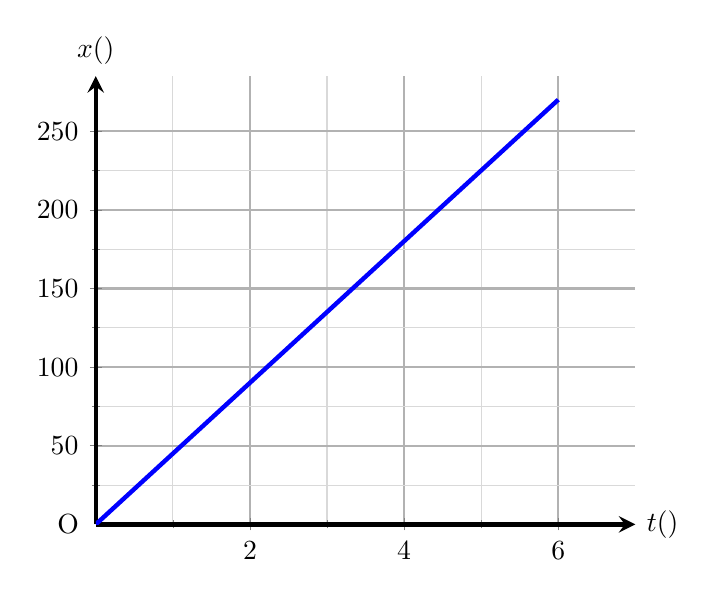
\begin{tikzpicture}  
			\begin{axis}[  ultra thick,
				xmin=0,  
				xmax=7,  
				xtick={0,2,...,6},
				ytick={0,50,...,250},
				minor x tick num=1,
				minor y tick num=1,
				ymin=0,  
				ymax=285, 
				samples=300,
				axis lines=center, 
				grid style={step=1, line width =0.4pt, color=gray!30!white},
				grid=both, %giới hạn ô lưới
				major grid style={line width=0.8pt,gray!60!white},
				xlabel=$\xsi{t}{\left(\si{\hour}\right)}$, 		ylabel=$\xsi{x}{\left(\si{\kilo\meter}\right)}$,
				every axis y label/.style={at=(current axis.above origin),anchor=south},  
				every axis x label/.style={at=(current axis.right of origin),anchor=west},  ] 
				\addplot [ultra thick, blue, smooth, domain=0:6] {45*x}; 
			\end{axis} 
			\node at (-0.35,0) {O}; 
		\end{tikzpicture}
		
	\end{center}
	\choice
	{\True $\SI{45}{\kilo\meter/\hour}$}
	{$\SI{43.75}{\kilo\meter/\hour}$}
	{$\SI{45.45}{\kilo\meter/\hour}$}
	{$\SI{50}{\kilo\meter/\hour}$}
	\loigiai{
		Tại $t=\SI{5}{\hour}$ thì $x=\SI{225}{\kilo\meter}$:
		$$\left|v\right|=\left|\dfrac{\Delta x}{\Delta t}\right|=\SI{45}{\kilo\meter/\hour}.$$	
	}
\end{ex}

% ===================================================================
\begin{ex}
	Một ô tô đang chạy với tốc độ $\SI{72}{\kilo\meter/\hour}$ thì hãm phanh chuyển động thẳng chậm dần đều với gia tốc có độ lớn $\SI{0.5}{\meter/\second^2}$. Quãng đường mà ô tô đã đi được trong 5 giây cuối trước khi dừng lại là
	\choice
	{$\SI{68.75}{\meter}$}
	{$\SI{81.25}{\meter}$}
	{$\SI{12.5}{\meter}$}
	{\True $\SI{6.25}{\meter}$}
	\loigiai{
		Đảo ngược thời gian sẽ thấy xe chuyển động nhanh dần đều với gia tốc $a=\SI{0.5}{\meter/\second^2}$, không vận tốc đầu. Lúc này, 5 giây cuối trở thành 5 giây đầu:
		$$s=\dfrac{1}{2}at^2=\dfrac{1}{2}\cdot0,5\cdot5^2=\SI{6.25}{\meter}.$$
	}
\end{ex}

\Closesolutionfile{ans}
\section{Câu trắc nghiệm đúng/sai} 
\textit{Thí sinh trả lời từ câu 1 đến câu 4. Trong mỗi ý \textbf{a)}, \textbf{b)}, \textbf{c)}, \textbf{d)} ở mỗi câu, thí sinh chọn đúng hoặc sai}
\setcounter{ex}{0}
\Opensolutionfile{ans}[ans/G10-5-TF]
% ===================================================================
\begin{ex}
	Một vật bắt đầu chuyển động từ điểm O đến điểm A, sau đó chuyển động về điểm B (như hình vẽ bên dưới).
	\begin{center}
		\includegraphics[width=0.4\linewidth]{../figs/D10-2-7}
	\end{center}
	\choiceTF[t]
	{Trong toàn bộ quá trình chuyển động nói trên, vector độ dịch chuyển của vật là $\vec{\mathrm{BO}}$}
	{\True Quãng đường và độ dịch chuyển của vật bằng nhau khi chuyển động từ điểm O đến điểm A}
	{\True Khi vật chuyển động từ điểm O đến điểm A rồi quay về điểm O thì quãng đường đi được là $\SI{6}{\meter}$}
	{\True Quãng đường và độ dịch chuyển của vật trong cả quá trình chuyển động lần lượt là $\SI{8}{\meter}$; $\SI{-2}{\meter}$}
	\loigiai{}
\end{ex}
% ===================================================================
\begin{ex}
	Một vật chuyển động thẳng có đồ thị vận tốc thời gian như hình bên dưới.
	\begin{center}
		\includegraphics[width=0.7\linewidth]{../figs/D10-2-8}
	\end{center}
	\choiceTF[t]
	{\True Vật đạt tốc độ lớn nhất tại B}
	{Trong quá trình AB, vật chuyển động thẳng đều}
	{Trong quá trình EF, vật đứng yên}
	{\True Độ lớn gia tốc tại D lớn hơn độ lớn gia tốc tại B}
	\loigiai{}
\end{ex}
% ===================================================================
\begin{ex}
	Hai xe 1 và 2 đang di chuyển trên 2 đường cao tốc song song. Tại thời điểm $t_0$, hai xe đồng thời vượt qua xe 3 đang dừng bên lề. Vào thời điểm này, tài xế xe 1 bấm phanh trong khi tài xế xe 3 lại bắt đầu tăng tốc. Hình bên dưới thể hiện vị trí của các xe trong 5 giây tiếp theo.
	\begin{center}
		\includegraphics[width=0.7\linewidth]{../figs/D10-2-10}
	\end{center}
	\choiceTF[t]
	{\True Tốc độ trung bình của xe 1 là $\SI{8}{\meter/\second}$}
	{\True Trong khoảng thời gian từ $t_1$ đến $t_2$ tốc độ trung bình của xe 2 bằng tốc độ trung bình của xe 3}
	{Trong khoảng thời gian từ $t_3$ đến $t_4$ tốc độ trung bình của xe 1 lớn hơn tốc độ trung bình của xe 2}
	{Nếu xe 3 chuyển động với gia tốc không đổi thì sau $\SI{6}{\second}$ xe 3 cách vị trí ban đầu $\SI{78}{\meter}$}
	\loigiai{
	\begin{itemchoice}
		\itemch Đúng.
		\itemch Đúng.
		\itemch Sai. Trong khoảng thời gian từ $t_3$ đến $t_4$ tốc độ trung bình của xe 1 nhỏ hơn tốc độ trung bình của xe 2
		\itemch Sai. Nếu xe 3 chuyển động với gia tốc không đổi thì sau $\SI{6}{\second}$ xe 3 cách vị trí ban đầu $\SI{72}{\meter}$.\\
		$$\dfrac{s_6}{s_5}=\dfrac{6^2}{5^2}\Rightarrow s_6=1,44s_5=1,44\cdot50=\SI{72}{\meter}.$$
	\end{itemchoice}
	}
\end{ex}
% ===================================================================
\begin{ex}
	Một thiết bị tạo ra các chấm trên một băng giấy chuyển động với khoảng thời gian giữa 2 chấm liên tiếp là $\SI{0.02}{\second}$. Hình 1, Hình 2 và Hình 3 biểu diễn kết 3 quả chuyển động thẳng của băng giấy. Mốc thời gian được chọn tại chấm 0.
	\begin{center}
		\includegraphics[width=0.4\linewidth]{../figs/D10-2-9}
	\end{center}
	\choiceTF[t]
	{\True Kết quả ở Hình 1 chứng tỏ băng giấy chuyển động thẳng đều}
	{Kết quả ở Hình 2 và Hình 3 chứng tỏ băng giấy chuyển động nhanh dần}
	{\True Tốc độ trung bình của băng giấy ở Hình 1 và Hình 2 trong $\SI{0.1}{\second}$ (tính từ mốc thời gian) là bằng nhau}
	{Độ lớn gia tốc của băng giấy ở Hình 2 lớn hơn độ lớn gia tốc của băng giấy ở Hình 3}
	\loigiai{
	\begin{itemchoice}
		\itemch Đúng.
		\itemch Sai. Hình 2 băng giấy chuyển động nhanh dần, Hình 3 băng giấy chuyển động chậm dần.
		\itemch Đúng.
		\itemch Sai. Chưa thể khẳng định vật chuyển động biến đổi đều nên chưa thể so sánh gia tốc trong 2 trường hợp.
	\end{itemchoice}
	}
\end{ex}
\Closesolutionfile{ans}
\section{Câu trắc nghiệm trả lời ngắn} \textit{Thí sinh trả lời từ câu 1 đến câu 6}
\setcounter{ex}{0}
\Opensolutionfile{ans}[ans/G10-5-TL]
% ===================================================================
\begin{ex}
	Chuyển động của hai viên bi $\mathrm{B}_1$ và $\mathrm{B}_2$ có đồ thị vận tốc thời gian như hình bên. Gọi $s_1$ và $s_2$ là quãng đường đi được tương ứng của $\mathrm{B}_1$ và $\mathrm{B}_2$ trong cùng thời gian kể từ thời điểm $t=\SI{0}{\second}$. Tỉ số $s_2/s_1$ là bao nhiêu? \textit{(Kết quả lấy đến 1 chữ số sau dấu phẩy thập phân)}.
	\begin{center}
		\begin{tikzpicture} 
			\coordinate (O)  at (0,0);
			\coordinate (t) at (4,0);
			\coordinate (v) at (0,4);
			\coordinate (A) at ($(O)+(30:3)$);
			\coordinate (B) at ($(O)+(60:3.5)$);
			\draw[line width=1pt, -latex] (O)--(v);
			\draw[line width=1pt, -latex] (O)--(t);
			\draw[line width=1.5pt, red] (O)--(A);
			\draw[line width=1.5pt, blue] (O)--(B);
			\node[left] at (O) {O};
			\node[above] at (t) {$t$};
			\node[left] at (v) {$v$};
			\tkzFillAngle[size=0.75cm,color=red, fill=red, opacity=0.25](t,O,A);
			\tkzLabelAngle[color=red,pos=1.2](t,O,A){$\SI{30}{\degree}$}
			\tkzMarkAngle[size=0.5cm,color=blue](t,O,B);
			\node[blue] at (0.75,0.7) {$\SI{60}{\degree}$};
			\node[above right, red] at (A) {$\mathrm{B}_2$};
			\node[above right, blue] at (B) {$\mathrm{B}_1$};
		\end{tikzpicture}
	\end{center}
	\shortans{0,3}
	\loigiai{
	$$\dfrac{s_2}{s_1}=\dfrac{\dfrac{1}{2}a_2t^2}{\dfrac{1}{2}a_1t^2}=\dfrac{a_2}{a_1}=\dfrac{\tan\SI{30}{\degree}}{\tan\SI{60}{\degree}}\approx0,3.$$
	}
\end{ex}
\textit{Dữ kiện sau đây được dùng chung cho câu 2 đến câu 5}\\
Bạn An thực hiện thí nghiệm đo tốc độ chuyển động thẳng với dụng cụ và sơ đồ bố trí thí nghiệm như hình bên dưới.
Trong đó, hai cổng quang điện A và B được đặt cách nhau $\SI{30}{\centi\meter}$ và được nối với đồng hồ đo thời gian hiện số (1) được đặt ở chế độ đo với sai số dụng cụ $\SI{0.01}{\second}$. Độ chia nhỏ nhất của thước đo (5) là $\SI{0.5}{\centi\meter}$.
\begin{center}
	\includegraphics[width=0.75\linewidth]{../figs/D10-2-6}
\end{center}
Bạn An thiết đặt đồng hồ đo thời gian hiện số ở chế độ A$\leftrightarrow$B để đo thời gian viên bi chuyển động kể từ khi chắn qua cổng quang A đến khi qua cổng quang B. Sau 5 lần đo, An ghi nhận được các giá trị thời gian chuyển động của viên bi như bảng bên dưới:
\begin{center}
	\begin{longtable}{|M{4cm}|M{2cm}|M{2cm}|M{2cm}|M{2cm}|M{2cm}|}
		\hline
		\thead{Lần đo}&1&2&3&4&5\\
		\hline
		\thead{Thời gian $\left(\si{\second}\right)$}& 4,75 & 4,68 & 4,73 & 4,68 & 4,70\\
		\hline
	\end{longtable}
\end{center}
\textit{* Lưu ý: Trong các phần tính toán bên dưới, các giá trị trung bình được lấy cùng bậc thập phân với giá trị đo.}
% ===============================================================
\begin{ex}
	Xác định thời gian chuyển động trung bình của viên bi \textit{(Kết quả tính theo đơn vị giây và làm tròn đến 3 CSCN)}.
	\shortans{4,71}
	\loigiai{
		Thời gian chuyển động trung bình của viên bi:
		$$\overline{t}=\dfrac{t_1+t_2+\dots+t_5}{5}=\SI{4.708}{\second}\approx\SI{4.71}{\second}.$$	
	}
\end{ex}
% ===============================================================
\begin{ex}
	Xác định sai số tương đối trong phép đo thời gian trên \textit{(Kết quả tính theo đơn vị $\si{\percent}$ và làm tròn đến 2 CSCN)}.
	\shortans{0,85}
	\loigiai{
		\begin{center}
			\begin{longtable}{|M{2cm}|M{4cm}|M{2cm}|}
				\hline
				\thead{Lần đo} & $\xsi{t}{\left(\second\right)}$ &$\xsi{\Delta t}{\left(\second\right)}$\\
				\hline
				1 & 4,75 &0,04 \\
				\hline
				2 & 4,68 & 0,03\\
				\hline
				3 & 4,73 & 0,02\\
				\hline
				4 & 4,68 & 0,03\\
				\hline
				5 & 4,70 & 0,01\\
				\hline
				\thead{TB}&4,71&0,03\\
				\hline
			\end{longtable}
		\end{center}
		Sai số tuyệt đối của phép đo thời gian:
		$$\Delta t=\overline{\Delta t}+\Delta t_{\text{dc}}=\SI{0.03}{\second}+\SI{0.01}{\second}=\SI{0.04}{\second}.$$
		Sai số tương đối của phép đo thời gian:
		$$\delta t=\dfrac{\Delta t}{\overline{t}}\cdot\SI{100}{\percent}=\dfrac{\SI{0.04}{\second}}{\SI{4.71}{\second}}\cdot\SI{100}{\percent}\approx\SI{0.85}{\percent}.$$}
\end{ex}
% ===============================================================
\begin{ex}
	Xác định tốc độ trung bình của viên bi trong thí nghiệm trên \textit{(Kết quả tính theo đơn vị $\si{\centi\meter/\second}$ và làm tròn đến 3 CSCN)}.
	\shortans{6,37}
	\loigiai{
		$$\overline{v}=\dfrac{\overline{s}}{\overline{t}}=\dfrac{\SI{30}{\centi\meter}}{\SI{4.71}{\second}}\approx\SI{6.37}{\centi\meter/\second}.$$
	}
\end{ex}
% ===============================================================
\begin{ex}
	Xác định sai số tuyệt đối trong phép đo tốc độ trung bình của viên bi \textit{(Kết quả tính theo đơn vị $\si{\centi\meter/\second}$ và làm tròn đến 2 CSCN)}.
	\shortans{0,11}
	\loigiai{
		ĐCNN của thước (5) là $\SI{0.5}{\centi\meter}$ nên sai số $\Delta s=\dfrac{\SI{0.5}{\centi\meter}}{2}=\SI{0.25}{\centi\meter}$.\\
		Sai số tuyệt đối trong phép đo tốc độ trung bình:
		$$\dfrac{\Delta v}{\overline{v}}=\dfrac{\Delta s}{\overline{s}}+\dfrac{\Delta t}{\overline{t}}\Rightarrow \Delta v=\left(\dfrac{\Delta s}{\overline{s}}+\dfrac{\Delta t}{\overline{t}}\right)\cdot\overline{v}=\left(\dfrac{\SI{0.25}{\centi\meter}}{\SI{30}{\centi\meter}}+\dfrac{\SI{0.04}{\second}}{\SI{4.71}{\second}}\right)\cdot\left(\SI{6.37}{\centi\meter/\second}\right)\approx\SI{0.11}{\centi\meter}.$$
	}
\end{ex}
	% ===============================================================
\begin{ex}
	Hố đen là một trong những đối tượng rất đặc biệt trong vũ trụ. Nguồn gốc ra đời của hố đen bắt nguồn từ sự suy sụp hấp dẫn của một vật thể khối lượng rất lớn vào một điểm kỳ dị và tạo ra quanh nó một vùng không - thời gian cong vô hạn, nơi mà không thứ gì có thể thoát ra từ đó, kể cả ánh sáng. 
	\begin{center}
		\begin{tabular}{M{7.5cm}M{7.5cm}}
			\includegraphics[width=0.7\linewidth]{../figs/D10-2-5}
			&\includegraphics[width=0.7\linewidth]{../figs/D10-2-4}\\
			\textit{Minh hoạ hố đen làm cong không - thời gian}& \textit{Ảnh hố đen chụp bởi Kính viễn vọng chân trời sự kiện (EHT) và công bố năm 2019} 
		\end{tabular}
	\end{center}
	Theo nhà vật lí học người Đức Karl Schwarzschild, một vật thể có kích thước bằng với bán kính giới hạn (bán kính Schwarzschild) thì nó sẽ trở thành một hố đen. Bán kính  Schwarzschild được cho bởi công thức:
	$$R_S=\dfrac{2GM}{c^2}$$
	Trong đó:
	\begin{itemize}
		\item $R_S$ là bán kính hấp dẫn Schwarzschild;
		\item $G$ là hằng số hấp dẫn;
		\item $M$ là khối lượng vật thể;
		\item $c$ là tốc độ ánh sáng trong chân không.
	\end{itemize}
	Trong công thức trên, hằng số hấp dẫn có thứ nguyên là $L^\alpha M^{-\beta}T^{-\gamma}$. Với $\alpha$, $\beta$, $\gamma$ là các số nguyên dương. Xác định giá trị của tổng $\alpha+\beta+\gamma$.
	
	\shortans{7}
	\loigiai{
		Ta có:
		$$G=\dfrac{1}{2}\dfrac{R_Sc^2}{M}.$$
		Phân tích thứ nguyên:
		$$\left[G\right]=\dfrac{\left[R_S\right]\times\left[c\right]^2}{\left[M\right]}=\dfrac{L\times\left(LT^{-1}\right)^2}{M}=L^3M^{-1}T^{-2}\Rightarrow \begin{cases}
			\alpha=3\\
			\beta=1\\
			\gamma=2
		\end{cases}.$$
	}
\end{ex}
\Closesolutionfile{ans}
\begin{center}
	\textbf{-- HẾT --}
\end{center}